% Options for packages loaded elsewhere
\PassOptionsToPackage{unicode}{hyperref}
\PassOptionsToPackage{hyphens}{url}
\PassOptionsToPackage{dvipsnames,svgnames,x11names}{xcolor}
%
\documentclass[
  11pt,
  a4paper,
]{article}

\usepackage{amsmath,amssymb}
\usepackage{setspace}
\usepackage{iftex}
\ifPDFTeX
  \usepackage[T1]{fontenc}
  \usepackage[utf8]{inputenc}
  \usepackage{textcomp} % provide euro and other symbols
\else % if luatex or xetex
  \usepackage{unicode-math}
  \defaultfontfeatures{Scale=MatchLowercase}
  \defaultfontfeatures[\rmfamily]{Ligatures=TeX,Scale=1}
\fi
\usepackage{lmodern}
\ifPDFTeX\else  
    % xetex/luatex font selection
\fi
% Use upquote if available, for straight quotes in verbatim environments
\IfFileExists{upquote.sty}{\usepackage{upquote}}{}
\IfFileExists{microtype.sty}{% use microtype if available
  \usepackage[]{microtype}
  \UseMicrotypeSet[protrusion]{basicmath} % disable protrusion for tt fonts
}{}
\makeatletter
\@ifundefined{KOMAClassName}{% if non-KOMA class
  \IfFileExists{parskip.sty}{%
    \usepackage{parskip}
  }{% else
    \setlength{\parindent}{0pt}
    \setlength{\parskip}{6pt plus 2pt minus 1pt}}
}{% if KOMA class
  \KOMAoptions{parskip=half}}
\makeatother
\usepackage{xcolor}
\usepackage[top=2.5cm,bottom=2.5cm,left=2.5cm,right=2.5cm]{geometry}
\ifLuaTeX
  \usepackage{luacolor}
  \usepackage[soul]{lua-ul}
\else
  \usepackage{soul}
  
\fi
\setlength{\emergencystretch}{3em} % prevent overfull lines
\setcounter{secnumdepth}{2}


\providecommand{\tightlist}{%
  \setlength{\itemsep}{0pt}\setlength{\parskip}{0pt}}\usepackage{longtable,booktabs,array}
\usepackage{calc} % for calculating minipage widths
% Correct order of tables after \paragraph or \subparagraph
\usepackage{etoolbox}
\makeatletter
\patchcmd\longtable{\par}{\if@noskipsec\mbox{}\fi\par}{}{}
\makeatother
% Allow footnotes in longtable head/foot
\IfFileExists{footnotehyper.sty}{\usepackage{footnotehyper}}{\usepackage{footnote}}
\makesavenoteenv{longtable}
\usepackage{graphicx}
\makeatletter
\newsavebox\pandoc@box
\newcommand*\pandocbounded[1]{% scales image to fit in text height/width
  \sbox\pandoc@box{#1}%
  \Gscale@div\@tempa{\textheight}{\dimexpr\ht\pandoc@box+\dp\pandoc@box\relax}%
  \Gscale@div\@tempb{\linewidth}{\wd\pandoc@box}%
  \ifdim\@tempb\p@<\@tempa\p@\let\@tempa\@tempb\fi% select the smaller of both
  \ifdim\@tempa\p@<\p@\scalebox{\@tempa}{\usebox\pandoc@box}%
  \else\usebox{\pandoc@box}%
  \fi%
}
% Set default figure placement to htbp
\def\fps@figure{htbp}
\makeatother

\usepackage{orcidlink}
\definecolor{mypink}{RGB}{219, 48, 122}
\makeatletter
\@ifpackageloaded{caption}{}{\usepackage{caption}}
\AtBeginDocument{%
\ifdefined\contentsname
  \renewcommand*\contentsname{Table of contents}
\else
  \newcommand\contentsname{Table of contents}
\fi
\ifdefined\listfigurename
  \renewcommand*\listfigurename{List of Figures}
\else
  \newcommand\listfigurename{List of Figures}
\fi
\ifdefined\listtablename
  \renewcommand*\listtablename{List of Tables}
\else
  \newcommand\listtablename{List of Tables}
\fi
\ifdefined\figurename
  \renewcommand*\figurename{Figure}
\else
  \newcommand\figurename{Figure}
\fi
\ifdefined\tablename
  \renewcommand*\tablename{Table}
\else
  \newcommand\tablename{Table}
\fi
}
\@ifpackageloaded{float}{}{\usepackage{float}}
\floatstyle{ruled}
\@ifundefined{c@chapter}{\newfloat{codelisting}{h}{lop}}{\newfloat{codelisting}{h}{lop}[chapter]}
\floatname{codelisting}{Listing}
\newcommand*\listoflistings{\listof{codelisting}{List of Listings}}
\makeatother
\makeatletter
\makeatother
\makeatletter
\@ifpackageloaded{caption}{}{\usepackage{caption}}
\@ifpackageloaded{subcaption}{}{\usepackage{subcaption}}
\makeatother

\usepackage[style=authoryear-comp,]{biblatex}
\addbibresource{references.bib}
\usepackage{bookmark}

\IfFileExists{xurl.sty}{\usepackage{xurl}}{} % add URL line breaks if available
\urlstyle{same} % disable monospaced font for URLs
\hypersetup{
  pdftitle={Git and GitHub Practical Guide},
  pdfauthor={Kunal Kapoor \textbar{} 34144161},
  colorlinks=true,
  linkcolor={blue},
  filecolor={Maroon},
  citecolor={Blue},
  urlcolor={Blue},
  pdfcreator={LaTeX via pandoc}}

%% CAPTIONS
\usepackage{caption}
\DeclareCaptionStyle{italic}[justification=centering]
 {labelfont={bf},textfont={it},labelsep=colon}
\captionsetup[figure]{style=italic,format=hang,singlelinecheck=true}
\captionsetup[table]{style=italic,format=hang,singlelinecheck=true}

%% FONT
\usepackage{bera}
\usepackage[charter]{mathdesign}
\usepackage[scale=0.9]{sourcecodepro}
\usepackage[lf,t]{FiraSans}

%% HEADERS AND FOOTERS
\usepackage{fancyhdr}
\pagestyle{fancy}
\rfoot{\Large\sffamily\raisebox{-0.1cm}{\textbf{\thepage}}}
\makeatletter
\lhead{\textsf{\expandafter{\@title}}}
\makeatother
\rhead{}
\cfoot{}
\setlength{\headheight}{15pt}
\renewcommand{\headrulewidth}{0.4pt}
\renewcommand{\footrulewidth}{0.4pt}
\fancypagestyle{plain}{%
\fancyhf{} % clear all header and footer fields
\fancyfoot[C]{\sffamily\thepage} % except the center
\renewcommand{\headrulewidth}{0pt}
\renewcommand{\footrulewidth}{0pt}}

%% MATHS
\usepackage{bm,amsmath}
\allowdisplaybreaks

%% GRAPHICS
\makeatletter
\def\fps@figure{htbp}
\makeatother
\setcounter{topnumber}{2}
\setcounter{bottomnumber}{2}
\setcounter{totalnumber}{4}
\renewcommand{\topfraction}{0.85}
\renewcommand{\bottomfraction}{0.85}
\renewcommand{\textfraction}{0.15}
\renewcommand{\floatpagefraction}{0.8}

%% SECTION TITLES
\usepackage[compact,sf,bf]{titlesec}
\titleformat{\section}[block]
  {\fontsize{15}{17}\bfseries\sffamily}
  {\thesection}
  {0.4em}{}
\titleformat{\subsection}[block]
  {\fontsize{12}{14}\bfseries\sffamily}
  {\thesubsection}
  {0.4em}{}
\titlespacing{\section}{0pt}{*5}{*1}
\titlespacing{\subsection}{0pt}{*2}{*0.2}
\titlespacing{\subsubsection}{0pt}{*1}{*0.1}

%% BIBLIOGRAPHY.

\makeatletter
\@ifpackageloaded{biblatex}{
\ExecuteBibliographyOptions{bibencoding=utf8,minnames=1,maxnames=3, maxbibnames=99,dashed=false,terseinits=true,giveninits=true,uniquename=false,uniquelist=false,doi=false, isbn=false,url=true,sortcites=false}
\DeclareFieldFormat{url}{\texttt{\url{#1}}}
\DeclareFieldFormat[article]{pages}{#1}
\DeclareFieldFormat[inproceedings]{pages}{\lowercase{pp.}#1}
\DeclareFieldFormat[incollection]{pages}{\lowercase{pp.}#1}
\DeclareFieldFormat[article]{volume}{\mkbibbold{#1}}
\DeclareFieldFormat[article]{number}{\mkbibparens{#1}}
\DeclareFieldFormat[article]{title}{\MakeCapital{#1}}
\DeclareFieldFormat[article]{url}{}
\DeclareFieldFormat[inproceedings]{title}{#1}
\DeclareFieldFormat{shorthandwidth}{#1}
\usepackage{xpatch}
\xpatchbibmacro{volume+number+eid}{\setunit*{\adddot}}{}{}{}
% Remove In: for an article.
\renewbibmacro{in:}{%
  \ifentrytype{article}{}{%
  \printtext{\bibstring{in}\intitlepunct}}}
\AtEveryBibitem{\clearfield{month}}
\AtEveryCitekey{\clearfield{month}}
\DeclareDelimFormat[cbx@textcite]{nameyeardelim}{\addspace}
\renewcommand*{\finalnamedelim}{\addspace\&\space}
}{}
\makeatother

%% PAGE BREAKING to avoid widows and orphans
\clubpenalty = 2000
\widowpenalty = 2000
\usepackage{microtype}
% Placement of logos

\RequirePackage[absolute,overlay]{textpos}
\setlength{\TPHorizModule}{1cm}
\setlength{\TPVertModule}{1cm}
\def\placefig#1#2#3#4{\begin{textblock}{.1}(#1,#2)\rlap{\includegraphics[#3]{#4}}\end{textblock}}

% Title and date

\title{Git and GitHub Practical Guide}
\date{7 May 2025}

\def\Date{\number\day}
\def\Month{\ifcase\month\or
 January\or February\or March\or April\or May\or June\or
 July\or August\or September\or October\or November\or December\fi}
\def\Year{\number\year}

% Working paper number and JEL codes

\makeatletter
\def\wp#1{\gdef\@wp{#1}}\def\@wp{??/??}
\def\jel#1{\gdef\@jel{#1}}\def\@jel{??}
\def\showjel{{\large\textsf{\textbf{JEL classification:}}~\@jel}}
\def\nojel{\def\showjel{}}
\makeatother

\nojel

% Title page

\makeatletter
\def\cover{{\sffamily\setcounter{page}{0}
        \thispagestyle{empty}
        \placefig{2}{1.5}{width=5cm}{monash2}
        \placefig{16.9}{1.5}{width=2.1cm}{MBSportrait}
        \begin{textblock}{7}(12.7,27.9)\hfill
        
\includegraphics[height=0.7cm]{AACSB}~~~
        
\includegraphics[height=0.7cm]{EQUIS}~~~
        
\includegraphics[height=0.7cm]{AMBA}
        \end{textblock}
        \vspace*{2.5cm}
        \begin{center}\Large
        Department of Econometrics and Business Statistics\\[.5cm]
        \end{center}\vspace{2cm}
        \begin{center}
        \fbox{\parbox{14cm}{\begin{onehalfspace}\centering\Huge\vspace*{0.3cm}
                \textsf{\textbf{\expandafter{\@title}}}\vspace{1cm}\par
                \LARGE
                \expandafter{\@author}
                \end{onehalfspace}
        }}
        \end{center}
        \vfill
                \begin{center}\Large
                \Month~\Year\\[1cm]

        \end{center}\vspace*{2cm}}}
        \def\addresses#1{\gdef\@addresses{#1}}\def\@addresses{??}
        \def\pageone{{\sffamily\setstretch{1}%
        \thispagestyle{empty}%
        \vbox to \textheight{%
        \raggedright\baselineskip=1.2cm
     {\fontsize{24.88}{30}\sffamily\textbf{\expandafter{\@title}}}
        \vspace{2cm}\par
        \hspace{1cm}\parbox{14cm}{\sffamily\large\@addresses}\vspace{1cm}\vfill
        \hspace{1cm}{\large\Date~\Month~\Year}\\[1cm]
        \hspace{1cm}\showjel\vss}}}
\def\blindtitle{{\sffamily
     \thispagestyle{plain}\raggedright\baselineskip=1.2cm
     {\fontsize{24.88}{30}\sffamily\textbf{\expandafter{\@title}}}\vspace{1cm}\par
        }}
\def\titlepage{{\cover}}

\def\blind{\def\titlepage{{\blindtitle}}\let\maketitle\blindtitle}
\def\titlepageonly{\def\titlepage{{\pageone\end{document}}}}
\def\nocover{\def\titlepage{{\pageone\newpage\blindtitle}}\let\maketitle\titlepage}
\let\maketitle\titlepage
\makeatother

% Authors


  \author{Kunal Kapoor \textbar{} 34144161}
  \addresses{%
    %
      \textbf{Kunal Kapoor \textbar{} 34144161}\\%
      %
      %
      \\[0.5cm]%
   %
   }%
   \lfoot{\sf 34144161: 7 May 2025}

% Keywords

\newenvironment{keywords}{\par\vspace{0.5cm}\noindent{\sffamily\textbf{Keywords:}}}{\vspace{0.25cm}\par\hrule\vspace{0.5cm}\par}

% Abstract
\renewenvironment{abstract}{\begin{minipage}{\textwidth}\parskip=1.4ex\noindent
\hrule\vspace{0.1cm}\par{\sffamily\textbf{\abstractname}}\newline\setstretch{1.5}}
  {\end{minipage}}
\begin{document}
\maketitle

\begin{abstract}
This guide provides a structured walkthrough of using Git and GitHub for
efficient version control and collaboration. It covers essential
concepts, practical commands, and workflows to help individuals track
changes, manage branches, resolve conflicts, and maintain organized
project histories.
\end{abstract}

    \vspace{0.25cm}\par\hrule\vspace{0.5cm}\par
  

\setstretch{1.5}
\section{Git Guide: Version Control and
Collaboration}\label{git-guide-version-control-and-collaboration}

\subsection{What is Git?}\label{what-is-git}

Git is a \textbf{distributed version control system} that tracks changes
in files and helps teams collaborate safely on projects.

With Git, you can:

\begin{itemize}
\item
  Save snapshots of your work (called \textbf{commits})
\item
  Restore previous versions when needed
\item
  Work on multiple ideas at once (using \textbf{branches})
\item
  Merge changes from different contributors
\item
  Experiment safely without disturbing the main project
\end{itemize}

Git is the most widely used version control system today, trusted by
individual developers, companies, and open-source communities worldwide.

\newpage

\subsection{Why Use Git?}\label{why-use-git}

Using Git offers major benefits:

\begin{itemize}
\item
  \textbf{Version Control:} Track every change made to your project
  files.
\item
  \textbf{Collaboration}: Multiple people can work on the same project
  without overwriting each other's changes.
\item
  \textbf{Backup:} Push your project to online services like GitHub to
  keep it safe.
\item
  \textbf{Experimentation:} Create branches to safely try new features
  without affecting the main project.
\item
  \textbf{Mistake Recovery:} Easily undo mistakes by rolling back to
  earlier commits.
\item
  \textbf{Transparency:} Clearly see who made changes, when, and why.
\end{itemize}

Whether working alone or with a team, Git makes your projects safer,
more organized, and more professional.

\newpage

\subsection{Key Concepts in GIT}\label{key-concepts-in-git}

\begin{longtable}[]{@{}
  >{\raggedright\arraybackslash}p{(\linewidth - 2\tabcolsep) * \real{0.1604}}
  >{\raggedright\arraybackslash}p{(\linewidth - 2\tabcolsep) * \real{0.8396}}@{}}
\caption{~Key concepts and terms used in Git, explained in simple
language.}\tabularnewline
\toprule\noalign{}
\begin{minipage}[b]{\linewidth}\raggedright
Term
\end{minipage} & \begin{minipage}[b]{\linewidth}\raggedright
Meaning
\end{minipage} \\
\midrule\noalign{}
\endfirsthead
\toprule\noalign{}
\begin{minipage}[b]{\linewidth}\raggedright
Term
\end{minipage} & \begin{minipage}[b]{\linewidth}\raggedright
Meaning
\end{minipage} \\
\midrule\noalign{}
\endhead
\bottomrule\noalign{}
\endlastfoot
\textbf{Repository} & A folder that Git tracks; contains project files
and the Git history. \\
\textbf{Commit} & A saved snapshot of your project at a specific point
in time. \\
\textbf{Branch} & A separate line of development; allows safe parallel
work. \\
\textbf{Merge} & Combining changes from different branches together. \\
\textbf{Conflict} & When two branches edit the same part of a file
differently; must be resolved manually. \\
\textbf{Remote} & A version of your repository hosted online (e.g.,
GitHub). \\
\textbf{Tag} & A fixed label for a specific commit, often used for
marking releases (e.g., v1.0). \\
\end{longtable}

\newpage

\subsection{Setting Up Git}\label{setting-up-git}

Before starting with Git, make sure you have the following:

\begin{itemize}
\tightlist
\item
  \textbf{Git Installed:}
\end{itemize}

Install Git on your computer.

→ You can download it from git-scm.com or install it through your
operating system's package manager (e.g., Homebrew on Mac, apt on Linux,
etc.).

\begin{itemize}
\tightlist
\item
  \textbf{GitHub Account:}
\end{itemize}

Create a free account at github.com to store your repositories online
and collaborate with others.

\begin{itemize}
\tightlist
\item
  \textbf{Code Editor:}
\end{itemize}

You can use any text editor or IDE (like Visual Studio Code, RStudio, or
even plain Notepad++) to work with Git projects.

Git itself does not depend on any specific software. \newpage

\subsection{Practical Walkthrough: Applying
Git}\label{practical-walkthrough-applying-git}

In this section, we apply Git basics through a real mini-project
example.

We will:

\begin{itemize}
\item
  Set up a project folder
\item
  Track changes with Git
\item
  Push to GitHub
\item
  Create branches
\item
  Handle conflicts
\item
  Tag versions
\end{itemize}

And more!

These steps cover the full cycle of using Git for version control and
collaboration.

\subsubsection{Step 1: Initialize Git Repository and Create Project
File}\label{step-1-initialize-git-repository-and-create-project-file}

First, we set up Git tracking inside our project folder and create our
first file.

Commands we ran in our command line interface

\begin{verbatim}
git init
\end{verbatim}

The above command Initializes Git tracking in the folder.

Then we create a file example.qmd (can be done through your code editor)
and knit it into an HTML output to confirm it works.

Step 1.2:

\begin{enumerate}
\def\labelenumi{\arabic{enumi}.}
\item
  Open your code editor (e.g., RStudio).
\item
  Create a new Quarto document (example.qmd).
\item
  Add simple content like a title and a few lines of text.
\item
  Save the file inside your project folder.
\item
  Render (knit) the example.qmd to produce an HTML file (e.g.,
  example.html).
\end{enumerate}

\begin{figure}[H]

{\centering \pandocbounded{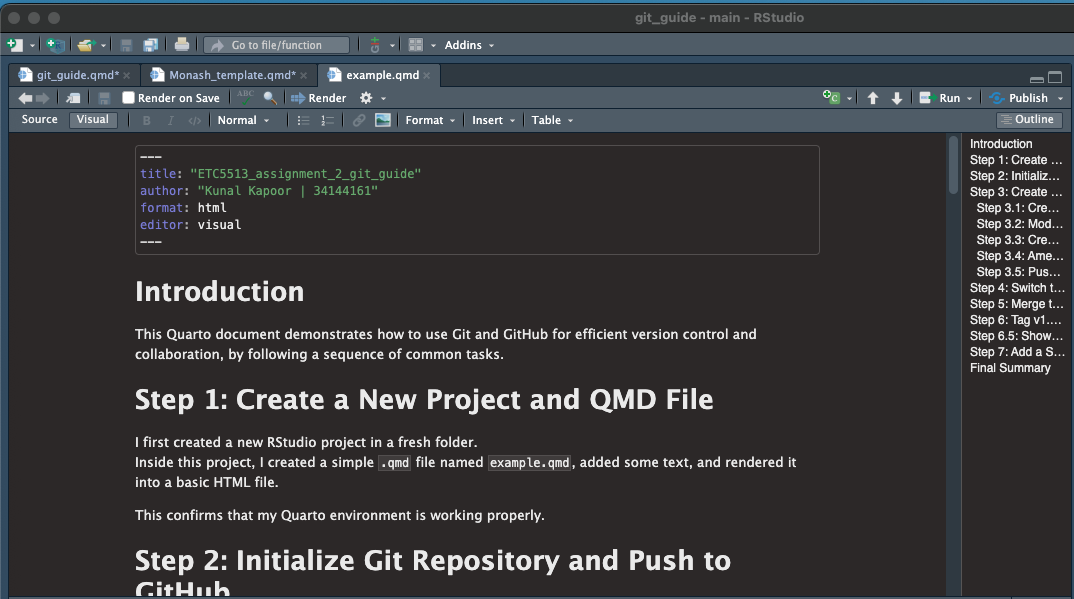
\includegraphics[keepaspectratio]{images/rstudio_working.png}}

}

\caption{File before rendering}

\end{figure}%

\begin{center}\rule{0.5\linewidth}{0.5pt}\end{center}

\begin{figure}[H]

{\centering \pandocbounded{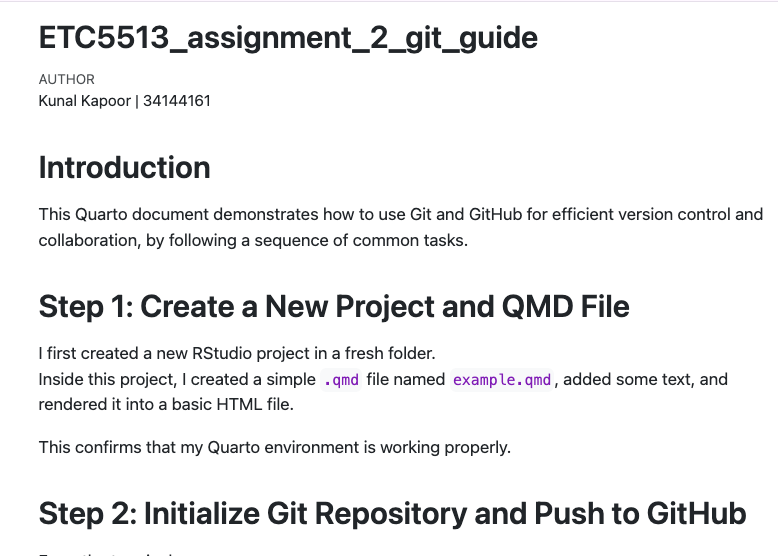
\includegraphics[keepaspectratio]{images/rendered_html.png}}

}

\caption{Rendered HTML}

\end{figure}%

\subsubsection{Step 2: First Commit}\label{step-2-first-commit}

We save our project's first version into Git history.

\textbf{Commands}:

\begin{verbatim}
git add example.qmd 
git commit -m "First Commit - Added example.qmd and rendered HTML files"
\end{verbatim}

This creates the first checkpoint of our project.

\textbf{Note}: Please run these above commands one by one \newpage

\subsubsection{Step 3: Link to GitHub and
Push}\label{step-3-link-to-github-and-push}

Now we connect our local project to GitHub and upload it.

\textbf{Commands}:

\begin{verbatim}
git remote add origin <your-repository-URL>
git push -u origin main
\end{verbatim}

This makes sure our work is backed up online.

\newpage

\subsubsection{Step 4: Create a New Branch and Make
Changes}\label{step-4-create-a-new-branch-and-make-changes}

We create a separate branch to work safely without disturbing the main
branch.

\textbf{Commands}:

\begin{verbatim}
git checkout -b testbranch
# Create and switch to a new branch called 'testbranch'
# Edit example.qmd (e.g., add a new line)
git add example.qmd
git commit -m "Step 3.2: Added a line to example.qmd in testbranch"
git push -u origin testbranch
\end{verbatim}

Changes are safely made inside testbranch.

\textbf{\emph{Note:}} Whenever you see \# followed by text in the
command examples, it is a comment. Comments are for humans to read ---
the computer ignores them when running commands.

\newpage

\subsubsection{Step 5: Add Data Folder and Amend Previous
Commit}\label{step-5-add-data-folder-and-amend-previous-commit}

We add a new folder data/ (e.g., containing Assignment 1 files) and
update our last commit to include it.

\textbf{Commands}:

\begin{verbatim}
mkdir data
# Create a new folder named 'data'
# Move your Assignment 1 data files into the 'data' folder manually
git add data/
# Stage the entire 'data' folder for the next commit
git commit --amend --no-edit
# Update the last commit to include the staged data folder without changing the commit message
git push --force
# Force push the amended commit to GitHub
\end{verbatim}

The previous commit now includes the new folder without making an extra
commit. \newpage

\subsubsection{Step 6: Modify Main Branch to Create
Conflict}\label{step-6-modify-main-branch-to-create-conflict}

We make different changes directly on main branch to simulate a merge
conflict later.

\textbf{Commands}:

\begin{verbatim}
git checkout main
# Switch back to the main branch
# Edit example.qmd (modify the same line differently)
git add example.qmd
# Stage the changes
git commit -m "creating a conflicting change in main branch"
# Save the conflicting changes
git push
# Push the conflicting changes to GitHub
\end{verbatim}

Now main and testbranch both have different edits to the same file.
\newpage

\subsubsection{Step 7: Merge Branches and Resolve
Conflict}\label{step-7-merge-branches-and-resolve-conflict}

We attempt to merge testbranch into main. Git detects the conflict, and
we fix it manually.

\textbf{Commands}:

\begin{verbatim}
git merge testbranch
# Attempt to merge 'testbranch' into 'main'
# Git will detect a conflict and stop the merge
# Open example.qmd manually
# Look for conflict markers like:
# <<<<<<< HEAD
# (your main branch content)
# =======
# (your testbranch content)
# >>>>>>> testbranch
# Decide which version to keep or combine them, then save the file

git add example.qmd
# Stage the resolved file

git commit -m "Fixed merge conflict between main and testbranch"
# Save the merge result

git push
# Push the resolved version to GitHub
\end{verbatim}

Changes from both branches are combined after resolving the conflict.
\newpage

\subsubsection{Step 8: Tagging a
Version}\label{step-8-tagging-a-version}

We mark the current state of the project as version 1.0.

\textbf{Commands}:

\begin{verbatim}
git tag -a v1.0 -m "Version 1.0 release"
git push origin v1.0
\end{verbatim}

Versioning helps you identify stable points in your project. \newpage

\subsubsection{Step 9: Show Commit Log in Condensed
Form}\label{step-9-show-commit-log-in-condensed-form}

We display a simple, one-line summary of the project's commit history.

\textbf{Commands}:

\begin{verbatim}
git log --oneline
# Shows a compact list of all commits
\end{verbatim}

\begin{figure}[H]

{\centering \pandocbounded{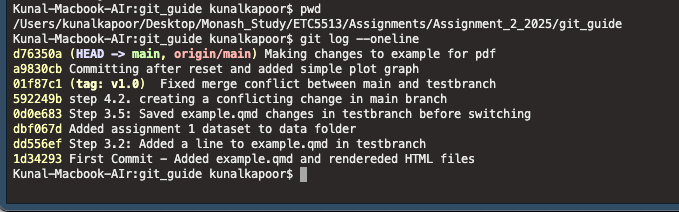
\includegraphics[keepaspectratio]{images/git_log_screenshot-min.png}}

}

\caption{Git log --oneline condensed form}

\end{figure}%

\newpage

\subsubsection{Step 10: Clean Up Old
Branch}\label{step-10-clean-up-old-branch}

We delete the testbranch locally and remotely since it's no longer
needed.

\textbf{Commands}:

\begin{verbatim}
git branch -d testbranch
git push origin --delete testbranch
\end{verbatim}

Keeping only necessary branches keeps the project tidy. \newpage

\subsubsection{Step 11: Undo a Commit (Without Losing
Changes)}\label{step-11-undo-a-commit-without-losing-changes}

Suppose we add a new section (like a plot) to example.qmd, but realize
we committed too early. We can undo the last commit while keeping
changes intact.

\textbf{Commands}:

\begin{verbatim}
# After editing and committing
git reset --soft HEAD~1
\end{verbatim}

The last commit is undone, but your edits remain staged, ready for a
better commit. \newpage

\section{Summary of Actions}\label{summary-of-actions}

By following these steps, you learned how to:

\begin{itemize}
\item
  Set up a Git repository
\item
  Track and save changes
\item
  Work safely using branches
\item
  Connect your project to a remote GitHub repository
\item
  Push and pull changes to/from GitHub
\item
  Handle merge conflicts
\item
  Tag versions
\item
  Manage commits and undo mistakes \newpage
\end{itemize}

\section{Git Commands Quick
Reference}\label{git-commands-quick-reference}

\begin{longtable}[]{@{}
  >{\raggedright\arraybackslash}p{(\linewidth - 4\tabcolsep) * \real{0.2831}}
  >{\raggedright\arraybackslash}p{(\linewidth - 4\tabcolsep) * \real{0.4398}}
  >{\raggedright\arraybackslash}p{(\linewidth - 4\tabcolsep) * \real{0.2711}}@{}}
\caption{Quick reference table summarizing important Git commands and
their purposes.}\tabularnewline
\toprule\noalign{}
\begin{minipage}[b]{\linewidth}\raggedright
\ul{\textbf{Git Command}}
\end{minipage} & \begin{minipage}[b]{\linewidth}\raggedright
\ul{\textbf{Meaning}}
\end{minipage} & \begin{minipage}[b]{\linewidth}\raggedright
\ul{\textbf{Why It's Useful}}
\end{minipage} \\
\midrule\noalign{}
\endfirsthead
\toprule\noalign{}
\begin{minipage}[b]{\linewidth}\raggedright
\ul{\textbf{Git Command}}
\end{minipage} & \begin{minipage}[b]{\linewidth}\raggedright
\ul{\textbf{Meaning}}
\end{minipage} & \begin{minipage}[b]{\linewidth}\raggedright
\ul{\textbf{Why It's Useful}}
\end{minipage} \\
\midrule\noalign{}
\endhead
\bottomrule\noalign{}
\endlastfoot
\texttt{git\ init} & Start tracking the project with Git & Begin version
control \\
\texttt{git\ status} & Check the status of changes & See staged,
unstaged, or untracked files \\
\texttt{git\ add\ filename} & Stage a specific file & Prepare file for
committing \\
\texttt{git\ add\ .} & Stage all changes in the working directory &
Quickly add everything for commit \\
\texttt{git\ commit\ -m\ "message"} & Save a snapshot of changes &
Record work into Git history \\
\texttt{git\ log} & Show commit history & View detailed list of
commits \\
\texttt{git\ log\ -\/-oneline} & Condensed commit history & View a brief
summary of commits \\
\texttt{git\ branch} & List all branches & Manage and view project
branches \\
\texttt{git\ branch\ branch\_name} & Create a new branch & Work
separately without affecting the main \\
\texttt{git\ switch\ branch\_name} & Switch to another branch & Move
between versions \\
\texttt{git\ switch\ -c\ branch\_name} & Create and switch to a new
branch & Shortcut to save time \\
\texttt{git\ merge\ branch\_name} & Merge another branch into current &
Combine features safely \\
\texttt{git\ push} & Upload commits to GitHub & Share work online \\
\texttt{git\ push\ -u\ origin\ main} & Push and track a new branch & Set
up branch tracking \\
\texttt{git\ pull} & Download and merge remote changes & Stay updated
with remote \\
\texttt{git\ tag\ -a\ v1.0\ -m\ "message"} & Create an annotated tag &
Mark important project points \\
\texttt{git\ reset\ -\/-soft\ HEAD\textasciitilde{}1} & Undo last commit
but keep changes staged & Correct mistakes without losing work \\
\texttt{git\ remote\ add\ origin\ url} & Connect local repo to GitHub &
Set up a remote repository \\
\texttt{git\ remote\ -v} & View remote connections & Confirm remote
links \\
\texttt{git\ remote\ remove\ origin} & Remove a GitHub link & Disconnect
remote repository \\
\texttt{git\ branch\ -d\ branch\_name} & Delete a local branch & Clean
up after merging \\
\texttt{git\ stash} & Temporarily save uncommitted work & Save work
without committing \\
\texttt{git\ stash\ pop} & Reapply stashed work & Restore work and
continue \\
\texttt{git\ revert\ commit\_id} & Undo a specific commit safely & Safe
undo for public history \\
\texttt{git\ rebase\ branch\_name} & Move branch commits onto another
branch & Simplify commit history \\
\texttt{git\ rebase\ -i\ HEAD\textasciitilde{}n}(squash inside rebase) &
Interactive rebase to squash commits Combine multiple commits into one &
\begin{minipage}[t]{\linewidth}\raggedright
Clean multiple commits\\
Tidy commit history\strut
\end{minipage} \\
\end{longtable}

\section{Conclusion}\label{conclusion}

Mastering Git provides a strong foundation for any collaborative or
individual project work. Whether you are coding, writing, or analyzing
data, Git ensures that your progress is organized, secure, and easy to
manage.


\printbibliography



\end{document}
